\documentclass{article}
\usepackage[UTF8]{ctex} % 用于中文排版
\usepackage{geometry}
\usepackage{indentfirst}
\usepackage{enumitem}

\usepackage{titling}    % 用于自定义标题页
\usepackage{graphicx}
\usepackage{float}

\usepackage{xcolor}
\usepackage{listings}

\usepackage{setspace}

% 页面几何设置
\geometry{a4paper, left=25mm, right=25mm, top=25mm, bottom=25mm}
% 取消首行缩进
\setlength{\parindent}{0pt}
% 行间距设置
\setstretch{1.5}
% 自定义字体大小
\newcommand{\fourhao}{\fontsize{14pt}{\baselineskip}\selectfont} % 四号字体
\newcommand{\xiaosihao}{\fontsize{12pt}{\baselineskip}\selectfont} % 小四号字体
\newcommand{\song}{\CJKfamily{song}}
% 设置代码块格式
\lstset{
    basicstyle = \footnotesize\ttfamily,                 % 设置行距,字体
    numbers = left,                                      % 在左侧显示行号
    numberstyle = \tiny \color{gray},                    % 设定行号格式
    keywordstyle = \bfseries \color[RGB]{40,40,255},     % 设定关键字颜色
    numberstyle = \footnotesize \color{darkgray},           
    commentstyle = \color[RGB]{0,96,96},                 % 设置代码注释的格式
    stringstyle = \color[RGB]{128,0,0},                  % 设置字符串格式
    frame = single,                                      % 不显示背景边框
    backgroundcolor = \color[RGB]{245,245,244},          % 设定背景颜色
    language=Verilog                                     % 设置语言
}
\raggedbottom   % 段落间留白, 避免排版时自动拉伸导致的行间距变化。
\begin{document}

% 封面页面
\begin{titlepage}
    \centering
    \vspace*{2cm}

    \Huge
    \textbf{课程名称:EDA 技术综合设计}

    \vspace{2cm}

    \LARGE
    设计报告名称:设计七\ 多功能数字钟

    \vspace{4cm}

    \centering
    \Large
    \begin{tabular}{rl}
        班级: & 通信214    \\
        姓名: & \ 王峤宇    \\
        学号: & \ 214022
    \end{tabular}

    \vfill

    \vspace{1cm}
\end{titlepage}

\newpage
% 第一部分
\section*{\fourhao 一、设计内容及原理}
\xiaosihao
\setstretch{1.5}
% 设计项目内容及设计原理,如真值表、状态表及状态转换图、文字说明等。
\subsection*{基础任务}
(1) 正常模式时,采用 24 小时制。显示时、分、秒。 \\
(2) 手动校准电路。按动时校准键,将系统置于校时状态,则计时 模块可用手动方式校准,每按一下校时键,时钟计数器加 1;按动 分校准键,将电路置于校分状态,以同样方式手动校分。\\
(3) 系统复位功能:复位控制只对秒计数复位,对分计数与小时计数无效。
\subsection*{提高内容}
\textbf{设计任务}:在基础任务基础上添加整点报时。仿中央人民广播电台整点报时功 能,从 59 分 50 秒起每隔 2 秒钟发出一次低音(512Hz)“嘟”信号 (信号鸣叫持续时间半秒,间隙 1 秒,连续 5 次,到达整点(00 分 00
秒时),发一次高音(1024 HZ)“哒”信号(信号持续时间半秒)。
\subsection*{拓展任务}
\textbf{任务要求}:在提高任务基础上添加闹钟功能。按下设置闹钟方式键,使系统工作于预置状态,此时显示器与时钟脱开,而与预置计数器相连,利用前面手动校时、校分方式进行预置,预置后回到正常计时模式。当计时计到预置的时间时,蜂鸣器发出闹钟信号,时间为一分钟,闹铃信号
可以用开关键 CLOSE“止闹”,正常情况下此开关键释放。\\
\begin{figure}[htbp]
    \centering
    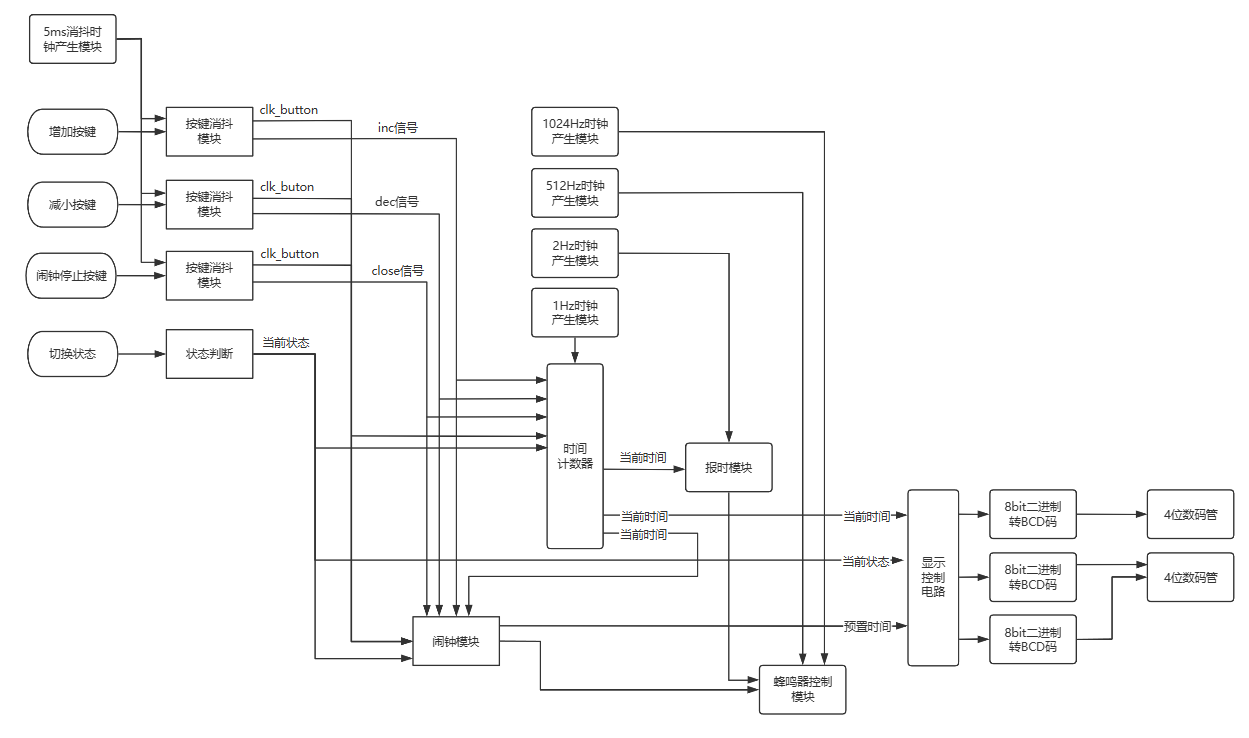
\includegraphics[width=0.8\textwidth]{image/2024-06-28-18-09-11.png}
    \caption{多功能数字钟系统的模块框图}
    \label{image_principle_1}
\end{figure}
最终设计得到支持时间加或减、报时和闹钟的数字钟的系统模块框图如图\ref{image_principle_1}所示。
% 第二部分
\section*{\fourhao 二、设计过程}
\xiaosihao
\setstretch{1.5}
% 从工程建立开始,一直到硬件调试。
% 按照基础任务、提高任务和拓展任务分别给出相应的源文件、仿真文件、约束文件
\subsection*{基础任务}
数字钟核心模块的源文件如下:
\begin{lstlisting}[language=Verilog, caption={数字钟模块}]
module digitalClock(
    input clk_1Hz,          /* 1Hz时钟信号 */
    input rst,              /* 高电平异步复位 */
    input hour_setting,     /* 校时 */
    input minute_setting,   /* 校分 */
    input setting_inc,      /* 校准增按键 */
    input setting_dec,      /* 校准减按键 */
    input clk_button,       /* 按键时钟 */
    output [4:0] hour,      /* 时 */
    output [5:0] minute,    /* 分 */
    output [5:0] secound    /* 秒 */
    );
    /* 设置状态 */
    assign st_setting = hour_setting || minute_setting; /* 校时模式 */
    assign clk_1Hz_buf = clk_1Hz & (!st_setting);       /* 秒计时计时时钟 */
    assign clk_buf = st_setting ? clk_button : clk_1Hz; /* 按键时钟和1Hz时钟切换 */

    /* 秒计数器 */
    reg [5:0] secound_r;
    assign secound_break = secound_r == 6'd59 ? 1'b1 : 1'b0;
    always @(posedge clk_1Hz_buf or posedge rst) begin
        if (rst) begin
            secound_r <= 6'b0;
        end
        else if (secound_r == 6'd59) begin
            secound_r <= 6'b0;
        end
        else if (st_setting == 1'b1) begin
            secound_r <= secound_r;
        end
        else begin
            secound_r <= secound_r + 1'b1;
        end
    end
    
    /* 分计数器 */
    reg [5:0] minute_r = 6'b0;
    assign minute_break = minute_r == 6'd59 ? 1'b1 : 1'b0;
    always @(posedge clk_buf) begin
        if (st_setting) begin
            case ({minute_setting, setting_inc, setting_dec})
                3'b110: begin
                    if (minute_r == 6'd59) begin
                        minute_r <= 6'b0;
                    end
                    else begin
                        minute_r <= minute_r + 1'b1;
                    end
                end
                3'b101: begin
                    if (minute_r == 6'd0) begin
                        minute_r <= 6'd59;
                    end
                    else begin
                        minute_r <= minute_r - 1'b1;
                    end
                end
                default: minute_r <= minute_r;
            endcase
        end
        else if (secound_break) begin
            if (minute_r == 6'd59) begin
                minute_r <= 6'b0;
            end
            else begin
                minute_r <= minute_r + 1'b1;
            end
        end
        else begin
            minute_r <= minute_r;
        end
    end

    /* 时计数器 */
    reg [4:0] hour_r = 5'b0;
    always @(posedge clk_buf) begin
        if (st_setting) begin
            case ({hour_setting, setting_inc, setting_dec})
                3'b110: begin
                    if (hour_r == 5'd23) begin
                        hour_r <= 5'b0;
                    end
                    else begin
                        hour_r <= hour_r + 1'b1;
                    end
                end
                3'b101: begin
                    if (hour_r == 5'd0) begin
                        hour_r <= 5'd23;
                    end
                    else begin
                        hour_r <= hour_r - 1'b1;
                    end
                end
                default: hour_r <= hour_r;
            endcase
        end
        else if (minute_break && secound_break) begin
            if (hour_r == 5'd23) begin
                hour_r <= 5'b0;
            end
            else begin
                hour_r <= hour_r + 1'b1;
            end
        end
        else begin
            hour_r <= hour_r;
        end
    end

    assign hour = hour_r;
    assign minute = minute_r;
    assign secound = secound_r;
endmodule    
\end{lstlisting}
时钟分频源码:
\begin{lstlisting}[language=Verilog, caption={任意分频}]
module clk_div_32bit(
    input clk,
    input rstn,
    input [31:0] step_freq,
    output clk_out
    );
    /* 相位累加器 */
    reg [31:0] cnt = 32'b0;
    always@(posedge clk or negedge rstn) begin
        if(!rstn)  
            cnt <= 32'b0;
        else  
            cnt <= cnt + step_freq;
    end
    /* 相位波形输出, 由于实现的是分频, 输出为50占空比的方波 */
    reg cnt_equal;
    always @(posedge clk or negedge rstn) begin
        if (!rstn) begin
            cnt_equal <= 1'b0;
        end else if(cnt < 32'h8000_0000) begin
            cnt_equal <= 1'b0;
        end else begin
            cnt_equal <= 1'b1;  
        end
    end
    assign clk_out = cnt_equal;
endmodule
\end{lstlisting}
8位二进制转BCD码:
\begin{lstlisting}[language=Verilog, caption={二进制转BCD码}]
module bin2bcd_8bit(
    input [7:0] bin, 
    output [11:0] bcd_12bit  /* 高中低BCD结果 */
    );

    integer i;
    reg [19:0] bcd_temp;
    always @(*) begin
        // 初始化, 直接移位三次
        bcd_temp = {9'b0, bin, 3'b0};
        // 逐位移位法
        for (i = 0; i < 5; i = i + 1'b1) begin
            // 如果BCD的每一部分 > 4,加3
            if (bcd_temp[11:8] > 4)
                bcd_temp[11:8] = bcd_temp[11:8] + 3;
            if (bcd_temp[15:12] > 4)
                bcd_temp[15:12] = bcd_temp[15:12] + 3;
            if (bcd_temp[19:16] > 4)
                bcd_temp[19:16] = bcd_temp[19:16] + 3;
            // 左移1位
            bcd_temp = {bcd_temp[18:0], 1'b0};
        end
    end
    assign bcd_12bit = bcd_temp[19-:12];
endmodule
\end{lstlisting}
按键消抖源文件如下:
\begin{lstlisting}[language=Verilog, caption={按键消抖}]
module button_fsm (
        input clk,                          /* 输入时钟 */
        input rst,                          /* 异步高电平复位信号 */
        input button_in,                    /* 输入开关信号 */
        output button_out                   /* 输出开关信号 */
    );
    //  状态声明
    localparam [2:0]
        zero    = 3'b000,
        wait1_1 = 3'b001,
        wait1_2 = 3'b010,
        wait1_3 = 3'b011,
        one     = 3'b100,
        wait0_1 = 3'b101,
        wait0_2 = 3'b110,
        wait0_3 = 3'b111;
    reg [2:0] state_cur, state_next;
    always@ (posedge clk or posedge rst) begin
        if (rst) begin
            state_cur <= zero;
        end
        else begin
            state_cur <= state_next;
        end
    end
    
    
    always @(*) begin
        case  (state_cur )
            zero : begin
                if (button_in)
                    state_next <= wait1_1;
                else
                    state_next <= zero;
            end
            wait1_1 : begin
                if (~button_in)
                    state_next <= zero ;
                else 
                    state_next <= wait1_2;
            end

            wait1_2 : begin
                if (~button_in)
                    state_next <= zero;
                else
                    state_next <= wait1_3;
            end

            wait1_3 : begin
                if (~button_in)
                    state_next <= zero;
                else
                    state_next <= one;
            end
            one : begin
                if (~button_in)
                    state_next <= wait0_1;
                else
                    state_next <= one;
            end
            wait0_1: begin
                if(button_in)
                    state_next <= one;
                else
                    state_next <= wait0_2;
            end
            wait0_2 : begin
                if(button_in)
                    state_next <= one;
                else
                    state_next <= wait0_3;
            end
            wait0_3 : begin
                if(button_in)
                    state_next <= one;
                else
                    state_next <= zero;
            end
            default :state_next <= zero;
        endcase
    end
    
    reg button_out_r;
    assign button_out = button_out_r;
    always @(posedge clk) begin
        case (state_next)
            one: begin
                if (state_cur == wait1_3) begin
                    button_out_r <= 1'b1;
                end
                else begin
                    button_out_r <= 1'b0;
                end
            end 
            default: button_out_r <= 1'b0;
        endcase
    end
endmodule
\end{lstlisting}
数码管显示代码:
\begin{lstlisting}[language=Verilog, caption={数码管显示}]
module scan_led_hex_disp_4(
    input clk, rst,
    input [3:0] hex0, hex1, hex2, hex3, /* 显存 */
    input [3:0] dp,
    output reg [3:0] an,
    output reg [7:0] sseg
    );

    localparam N = 16 + 2;              /* 100MHz时钟分频, 100Mhz/ 2^16 */         
    reg [N-1:0] regN;

    always @(posedge clk, posedge rst) begin
        if (rst)
            regN <= 0;
        else 
            regN <= regN + 1;
    end

    always @(*) begin
        case (regN[N-1:N-2])
            2'b00: begin
                an <= 4'b0001;
                sseg[6:0] <= dt_translate(hex0);
                sseg[7] <= dp[3];
            end
            2'b01: begin
                an <= 4'b0010;
                sseg[6:0] <= dt_translate(hex1);
                sseg[7] <= dp[2];
            end
            2'b10: begin
                an <= 4'b0100;
                sseg[6:0] <= dt_translate(hex2);
                sseg[7] <= dp[1];
            end
            2'b11: begin
                an <= 4'b1000;
                sseg[6:0] <= dt_translate(hex3);
                sseg[7] <= dp[0];
            end 
        endcase
    end

    function [6:0] dt_translate;
        input [3:0] data;
        begin
            case(data)
                4'd0: dt_translate = 7'b1111110;     //number 0 -> 0x7e
                4'd1: dt_translate = 7'b0110000;     //number 1 -> 0x30
                4'd2: dt_translate = 7'b1101101;     //number 2 -> 0x6d
                4'd3: dt_translate = 7'b1111001;     //number 3 -> 0x79
                4'd4: dt_translate = 7'b0110011;     //number 4 -> 0x33
                4'd5: dt_translate = 7'b1011011;     //number 5 -> 0x5b
                4'd6: dt_translate = 7'b1011111;     //number 6 -> 0x5f
                4'd7: dt_translate = 7'b1110000;     //number 7 -> 0x70
                4'd8: dt_translate = 7'b1111111;     //number 8 -> 0x7f
                4'd9: dt_translate = 7'b1111011;     //number 9 -> 0x7b
                default: dt_translate = 7'b0000000;  //不显示
            endcase
        end
    endfunction
endmodule    
\end{lstlisting}
top文件如下:
\begin{lstlisting}[language=Verilog, caption={top源文件}]
// `define STIMULATION
module digitalClock_top(
    input sys_clk,              /* 100MHz时钟信号 */
    input rst,                  /* 高电平异步复位 */
    input hour_setting,         /* 校时模式 */
    input minute_setting,       /* 校分模式 */
    input alarm_setting,        /* 闹钟设置 */
    input button_inc,           /* 校准增按键 */
    input button_dec,           /* 校准减按键 */
    input button_close,         /* 闹钟停止 */
    output [7:0] sseg1, sseg2,  /* 八段数码管 */
    output [3:0] an1, an2       /* 数码管片选信号 */
    );
    
    `ifdef STIMULATION
    assign clk_1Hz = sys_clk;
    `else
    wire clk_1Hz;
    /* 产生1.00117Hz信号 */
    clk_div_32bit  clk_div_32bit_inst_1 (
        .clk(sys_clk),
        .rstn(!rst),
        .step_freq(32'd43),
        .clk_out(clk_1Hz)
    );
    `endif
    
    wire clk_button;
    /* 产生5ms, 200.001Hz的按键时钟 */
    clk_div_32bit  clk_div_32bit_inst_2 (
        .clk(sys_clk),
        .rstn(!rst),
        .step_freq(32'd8590),
        .clk_out(clk_button)
    );

    button_fsm  button_fsm_inst_1 (
        .clk(clk_button),
        .rst(rst),
        .button_in(button_inc),
        .button_out(inc_buf)
    );

    button_fsm  button_fsm_inst_2 (
        .clk(clk_button),
        .rst(rst),
        .button_in(button_dec),
        .button_out(dec_buf)
    );

    button_fsm  button_fsm_inst_3 (
        .clk(clk_button),
        .rst(rst),
        .button_in(button_close),
        .button_out(close_buf)
    );

    wire [4:0] hour;
    wire [5:0] minute, secound;
    digitalClock  digitalClock_inst (
        .clk_1Hz(clk_1Hz),
        .rst(rst),
        .hour_setting(hour_setting & !alarm_setting),
        .minute_setting(minute_setting & !alarm_setting),
        .setting_inc(inc_buf), .setting_dec(dec_buf),
        .clk_button(clk_button),
        .hour(hour),
        .minute(minute),
        .secound(secound)
    );

    /* 数码管显示 */
    wire [3:0] dsp_buffer_1[0:1];
    wire [3:0] dsp_buffer_2[0:3];

    bin2bcd_8bit  bin2bcd_8bit_inst_1 (
        .bin(hour),
        .bcd_12bit({dsp_buffer_1[0], dsp_buffer_1[1]})
    );

    bin2bcd_8bit  bin2bcd_8bit_inst_2 (
        .bin(minute),
        .bcd_12bit({dsp_buffer_2[0], dsp_buffer_2[1]})
    );

    bin2bcd_8bit  bin2bcd_8bit_inst_3 (
        .bin(secound),
        .bcd_12bit({dsp_buffer_2[2], dsp_buffer_2[3]})
    );
    
    /* 第一个四位数码管 */
    scan_led_hex_disp_4  scan_led_hex_disp_4_inst_1 (
        .clk(sys_clk), .rst(rst),
        .hex0(4'd10), .hex1(4'd10),
        .hex2(dsp_buffer_1[0]), .hex3(dsp_buffer_1[1]),
        .dp(4'b0000), .an(an1), .sseg(sseg1)
    );
    /* 第二个四位数码管 */
    scan_led_hex_disp_4  scan_led_hex_disp_4_inst_2 (
        .clk(sys_clk), .rst(rst),
        .hex0(dsp_buffer_2[0]), .hex1(dsp_buffer_2[1]),
        .hex2(dsp_buffer_2[2]), .hex3(dsp_buffer_2[3]),
        .dp(4'b0000), .an(an2), .sseg(sseg2)
    );
endmodule
\end{lstlisting}
基础任务部分校准功能的仿真文件如下:
\begin{lstlisting}[language=Verilog, caption={校准仿真}]
module diditalClock_tb;
    reg  clk_1Hz;
    reg  rst;
    reg  hour_setting;
    reg  minute_setting;
    reg  setting_inc;
    reg  setting_dec;
    wire [4:0] hour;
    wire [5:0] minute;
    wire [5:0] secound;
    initial begin
        clk_1Hz = 1'b1;
        rst = 1'b0;
        hour_setting = 1'b0;
        minute_setting = 1'b0;
        setting_dec = 1'b0;
        setting_inc = 1'b0;
        #10;
        rst = 1'b1;
        #10;
        rst = 1'b0;
        wait(hour == 5'd1);
        hour_setting = 1'b1;
        #10;
        setting_inc = 1;
        #10;
        setting_inc = 0;
    end
    
    digitalClock  digitalClock_inst (
        .clk_1Hz(clk_1Hz),
        .rst(rst),
        .hour_setting(hour_setting),
        .minute_setting(minute_setting),
        .setting_inc(setting_inc),
        .setting_dec(setting_dec),
        .hour(hour),
        .minute(minute),
        .secound(secound)
    );

    always #5  clk_1Hz = ! clk_1Hz ;

endmodule
\end{lstlisting}
top仿真文件如下:
\begin{lstlisting}[language=Verilog, caption={top仿真文件}]
module top_tb;
    reg  sys_clk;
    reg  rst;
    reg  hour_setting;
    reg  minute_setting;
    reg  alarm_setting;
    reg  button_inc;
    reg  button_dec;
    reg  button_close;
    wire [7:0] sseg1;
    wire [7:0] sseg2;
    wire [3:0] an1;
    wire [3:0] an2;
    initial begin
        sys_clk = 1'b0;
        rst = 1'b0;
        #10;
        rst = 1'b1;
        #10;
        rst = 1'b0;
        {hour_setting, minute_setting, alarm_setting} = 3'b000;
        {button_inc, button_dec, button_close} = 3'b000;
        
        #100;
        hour_setting = 1'b1;
        #10;
        button_inc = 1'b1;
    end



    digitalClock_top  digitalClock_top_inst (
        .sys_clk(sys_clk),
        .rst(rst),
        .hour_setting(hour_setting),
        .minute_setting(minute_setting),
        .alarm_setting(alarm_setting),
        .button_inc(button_inc),
        .button_dec(button_dec),
        .button_close(button_close),
        .sseg1(sseg1),
        .sseg2(sseg2),
        .an1(an1),
        .an2(an2)
    );

    always #5  sys_clk = !sys_clk ;

endmodule
\end{lstlisting}
约束文件如下:
\begin{lstlisting}[language=Verilog, caption={约束文件}]
/* 100MHz时钟信号 */
set_property -dict {PACKAGE_PIN P17 IOSTANDARD LVCMOS33} [get_ports sys_clk]
/* 复位信号 */
set_property -dict {PACKAGE_PIN R11 IOSTANDARD LVCMOS33} [get_ports rst]
/* 按键开关 */
set_property -dict {PACKAGE_PIN U4 IOSTANDARD LVCMOS33} [get_ports button_inc]
set_property -dict {PACKAGE_PIN R17 IOSTANDARD LVCMOS33} [get_ports button_dec]
set_property -dict {PACKAGE_PIN R15 IOSTANDARD LVCMOS33} [get_ports button_close]
/* 拨码开关 */
set_property -dict {PACKAGE_PIN P5 IOSTANDARD LVCMOS33} [get_ports hour_setting]
set_property -dict {PACKAGE_PIN P4 IOSTANDARD LVCMOS33} [get_ports minute_setting]
set_property -dict {PACKAGE_PIN P3 IOSTANDARD LVCMOS33} [get_ports alarm_setting]
/* 数码管 */
set_property -dict {PACKAGE_PIN G2 IOSTANDARD LVCMOS33} [get_ports {an1[0]}]
set_property -dict {PACKAGE_PIN C2 IOSTANDARD LVCMOS33} [get_ports {an1[1]}]
set_property -dict {PACKAGE_PIN C1 IOSTANDARD LVCMOS33} [get_ports {an1[2]}]
set_property -dict {PACKAGE_PIN H1 IOSTANDARD LVCMOS33} [get_ports {an1[3]}]
set_property -dict {PACKAGE_PIN G6 IOSTANDARD LVCMOS33} [get_ports {an2[3]}]
set_property -dict {PACKAGE_PIN E1 IOSTANDARD LVCMOS33} [get_ports {an2[2]}]
set_property -dict {PACKAGE_PIN F1 IOSTANDARD LVCMOS33} [get_ports {an2[1]}]
set_property -dict {PACKAGE_PIN G1 IOSTANDARD LVCMOS33} [get_ports {an2[0]}]
set_property -dict {PACKAGE_PIN D5 IOSTANDARD LVCMOS33} [get_ports {sseg1[7]}]
set_property -dict {PACKAGE_PIN B4 IOSTANDARD LVCMOS33} [get_ports {sseg1[6]}]
set_property -dict {PACKAGE_PIN A4 IOSTANDARD LVCMOS33} [get_ports {sseg1[5]}]
set_property -dict {PACKAGE_PIN A3 IOSTANDARD LVCMOS33} [get_ports {sseg1[4]}]
set_property -dict {PACKAGE_PIN B1 IOSTANDARD LVCMOS33} [get_ports {sseg1[3]}]
set_property -dict {PACKAGE_PIN A1 IOSTANDARD LVCMOS33} [get_ports {sseg1[2]}]
set_property -dict {PACKAGE_PIN B3 IOSTANDARD LVCMOS33} [get_ports {sseg1[1]}]
set_property -dict {PACKAGE_PIN B2 IOSTANDARD LVCMOS33} [get_ports {sseg1[0]}]
set_property -dict {PACKAGE_PIN H2 IOSTANDARD LVCMOS33} [get_ports {sseg2[7]}]
set_property -dict {PACKAGE_PIN D4 IOSTANDARD LVCMOS33} [get_ports {sseg2[6]}]
set_property -dict {PACKAGE_PIN E3 IOSTANDARD LVCMOS33} [get_ports {sseg2[5]}]
set_property -dict {PACKAGE_PIN D3 IOSTANDARD LVCMOS33} [get_ports {sseg2[4]}]
set_property -dict {PACKAGE_PIN F4 IOSTANDARD LVCMOS33} [get_ports {sseg2[3]}]
set_property -dict {PACKAGE_PIN F3 IOSTANDARD LVCMOS33} [get_ports {sseg2[2]}]
set_property -dict {PACKAGE_PIN E2 IOSTANDARD LVCMOS33} [get_ports {sseg2[1]}]
set_property -dict {PACKAGE_PIN D2 IOSTANDARD LVCMOS33} [get_ports {sseg2[0]}]
\end{lstlisting}
\subsection*{提高任务}
报时模块如下:
\begin{lstlisting}[language=Verilog, caption={报时模块}]
module tellTime(
    input clk_1024Hz,         /* 1024Hz时钟信号 */
    input rst,              /* 异步高电平复位 */
    input [4:0] hour,       /* 时 */
    input [5:0] minute,     /* 分 */
    input [5:0] secound,    /* 秒 */
    output beepCtrl         /* 蜂鸣器控制信号 */
    );
    localparam [1:0]
        st_normal  = 2'b00, /* 正常状态 */
        st_closing = 2'b01, /* 即将整点 */
        st_closed  = 2'b11; /* 整点 */
    reg [1:0] st_cur, st_nxt;

    /* 二分频产生512Hz的蜂鸣器控制信号 */
    reg clk_512Hz;
    always @(posedge clk_1024Hz or posedge rst) begin
        if (rst) begin
            clk_512Hz <= 1'b0;
        end
        else begin
            clk_512Hz <= clk_512Hz + 1'b1;
        end
    end

    /* 512Hz分频产生2Hz信号, 分频2^8 */
    reg [7:0] cnt1;
    assign clk_2Hz = cnt1[7];
    always @(posedge clk_512Hz or posedge rst) begin
        if (rst) begin
            cnt1 <= 8'b0;
        end
        else begin
            cnt1 <= cnt1 + 1'b1;
        end
    end

    /* 状态转移 */
    always @(posedge clk_2Hz or posedge rst) begin
        if (rst) begin
            st_cur <= st_normal;
        end
        else begin
            st_cur <= st_nxt;
        end
    end

    reg [1:0] cnt2;
    always @(posedge clk_2Hz or posedge rst) begin
        if (rst) begin
            cnt2 <= 2'b0;
        end
        else if (st_cur == st_closing || st_cur == st_closed)begin
            cnt2 <= cnt2 + 1'b1;
        end
        else begin
            cnt2 <= 2'b0;
        end
    end

    /* 次态输出 */
    always @(*) begin
        case (st_cur)
            st_normal: begin
                if (minute == 6'd59 && secound == 6'd50) begin
                    st_nxt <= st_closing;
                end
                else begin
                    st_nxt <= st_normal;
                end
            end
            st_closing: begin
                if (secound == 6'd0) begin
                    st_nxt <= st_closed;
                end
                else begin
                    st_nxt <= st_closing;
                end
            end
            st_closed: begin
                if (secound == 6'd1) begin
                    st_nxt <= st_normal;
                end
                else begin
                    st_nxt <= st_closed;
                end
            end
            default: st_nxt <= st_normal;
        endcase
    end
    /*  信号输出 */
    reg beepCtrl_r;
    always @(*) begin
        case (st_cur)
            st_normal : beepCtrl_r <= 1'b0;
            st_closing : beepCtrl_r <= cnt2 == 2'b00 ? clk_512Hz : 1'b0;
            st_closed : beepCtrl_r <= cnt2 == 2'b00 ? clk_1024Hz : 1'b0;
            default: beepCtrl_r <= 1'b0;
        endcase
    end
    assign beepCtrl = beepCtrl_r;
endmodule
\end{lstlisting}
报时模块的仿真文件如下:
\begin{lstlisting}[language=Verilog, caption={报时模块仿真文件}]
`timescale 1ns / 1ns

module tellTime_tb;
    reg  clk_1024Hz;
    reg  rst;
    reg [4:0] hour;
    reg [5:0] minute;
    reg [5:0] secound;
    wire  beepCtrl;

    initial begin
        clk_1024Hz = 1'b0;
        rst = 1'b0;
        #10;
        rst = 1'b1;
        #10;
        rst = 1'b0;
        hour = 5'd0;
        minute = 6'd59;
        secound = 6'd49;
    end
    integer i = 0;
    always @(posedge clk_1024Hz) begin
        i = i + 1;
        if (i == 1024) begin
            if (secound < 6'd59) begin
                secound = secound + 1;
                i = 0;
            end
            else begin
                hour = hour + 1;
                secound = 0;
                minute = 0;
                #10000;
                $finish;
            end
        end
    end
    tellTime  tellTime_inst (
        .clk_1024Hz(clk_1024Hz),
        .rst(rst),
        .hour(hour),
        .minute(minute),
        .secound(secound),
        .beepCtrl(beepCtrl)
    );

    always #5 clk_1024Hz = !clk_1024Hz ;

endmodule
\end{lstlisting}
增加报时模块后的top文件如下:
\begin{lstlisting}[language=Verilog, caption={添加报时模块后的Top文件}]
// `define STIMULATION
module digitalClock_top(
    input sys_clk,              /* 100MHz时钟信号 */
    input rst,                  /* 高电平异步复位 */
    input hour_setting,         /* 校时模式 */
    input minute_setting,       /* 校分模式 */
    input alarm_setting,        /* 闹钟设置 */
    input button_inc,           /* 校准增按键 */
    input button_dec,           /* 校准减按键 */
    input button_close,         /* 闹钟停止 */
    output beepCtrl,            /* 蜂鸣器信号输出 */
    output [7:0] sseg1, sseg2,  /* 八段数码管 */
    output [3:0] an1, an2       /* 数码管片选信号 */
    );
    
    `ifdef STIMULATION
    assign clk_1Hz = sys_clk;
    `else
    wire clk_1Hz;
    /* 产生1.00117Hz信号 */
    clk_div_32bit  clk_div_32bit_inst_1 (
        .clk(sys_clk),
        .rstn(!rst),
        .step_freq(32'd43),
        .clk_out(clk_1Hz)
    );
    `endif
    
    wire clk_button;
    /* 产生5ms, 200.001Hz的按键时钟 */
    clk_div_32bit  clk_div_32bit_inst_2 (
        .clk(sys_clk),
        .rstn(!rst),
        .step_freq(32'd8590),
        .clk_out(clk_button)
    );

    /* 产生1023.98Hz的蜂鸣器控制信号 */
    wire clk_1024Hz;
    clk_div_32bit  clk_div_32bit_inst_3 (
        .clk(sys_clk),
        .rstn(!rst),
        .step_freq(32'd43980),
        .clk_out(clk_1024Hz)
    );

    button_fsm  button_fsm_inst_1 (
        .clk(clk_button),
        .rst(rst),
        .button_in(button_inc),
        .button_out(inc_buf)
    );

    button_fsm  button_fsm_inst_2 (
        .clk(clk_button),
        .rst(rst),
        .button_in(button_dec),
        .button_out(dec_buf)
    );

    button_fsm  button_fsm_inst_3 (
        .clk(clk_button),
        .rst(rst),
        .button_in(button_close),
        .button_out(close_buf)
    );

    wire [4:0] hour;
    wire [5:0] minute, secound;
    digitalClock  digitalClock_inst (
        .clk_1Hz(clk_1Hz),
        .rst(rst),
        .hour_setting(hour_setting & !alarm_setting),
        .minute_setting(minute_setting & !alarm_setting),
        .setting_inc(inc_buf), .setting_dec(dec_buf),
        .clk_button(clk_button),
        .hour(hour),
        .minute(minute),
        .secound(secound)
    );
    
    /* 报时模块的例化 */
    tellTime  tellTime_inst (
        .clk_1024Hz(clk_1024Hz),
        .rst(rst),
        .hour(hour),
        .minute(minute),
        .secound(secound),
        .beepCtrl(beepCtrl)
    );

    /* 数码管显示 */
    wire [3:0] dsp_buffer_1[0:1];
    wire [3:0] dsp_buffer_2[0:3];
    bin2bcd_8bit  bin2bcd_8bit_inst_1 (
        .bin(hour),
        .bcd_12bit({dsp_buffer_1[0], dsp_buffer_1[1]})
    );

    bin2bcd_8bit  bin2bcd_8bit_inst_2 (
        .bin(minute),
        .bcd_12bit({dsp_buffer_2[0], dsp_buffer_2[1]})
    );

    bin2bcd_8bit  bin2bcd_8bit_inst_3 (
        .bin(secound),
        .bcd_12bit({dsp_buffer_2[2], dsp_buffer_2[3]})
    );
    
    /* 第一个四位数码管 */
    scan_led_hex_disp_4  scan_led_hex_disp_4_inst_1 (
        .clk(sys_clk), .rst(rst),
        .hex0(4'd10), .hex1(4'd10),
        .hex2(dsp_buffer_1[0]), .hex3(dsp_buffer_1[1]),
        .dp(4'b0001), .an(an1), .sseg(sseg1)
    );
    /* 第二个四位数码管 */
    scan_led_hex_disp_4  scan_led_hex_disp_4_inst_2 (
        .clk(sys_clk), .rst(rst),
        .hex0(dsp_buffer_2[0]), .hex1(dsp_buffer_2[1]),
        .hex2(dsp_buffer_2[2]), .hex3(dsp_buffer_2[3]),
        .dp(4'b0100), .an(an2), .sseg(sseg2)
    );
endmodule
\end{lstlisting}
\subsection*{拓展任务}
增加闹钟模块后的top文件如下:
\begin{lstlisting}[language=Verilog, caption={增加闹钟模块后的top文件}]
module digitalClock_top(
    input sys_clk,              /* 100MHz时钟信号 */
    input rst,                  /* 高电平异步复位 */
    input hour_setting,         /* 校时模式 */
    input minute_setting,       /* 校分模式 */
    input alarm_setting,        /* 闹钟设置 */
    input button_inc,           /* 校准增按键 */
    input button_dec,           /* 校准减按键 */
    input button_close,         /* 闹钟停止 */
    output beepCtrl,            /* 蜂鸣器信号输出 */
    output [7:0] sseg1, sseg2,  /* 八段数码管 */
    output [3:0] an1, an2       /* 数码管片选信号 */
    );
    
    `ifdef STIMULATION
    assign clk_1Hz = sys_clk;
    `else
    wire clk_1Hz;
    /* 产生1.00117Hz信号 */
    clk_div_32bit  clk_div_32bit_inst_1 (
        .clk(sys_clk),
        .rstn(!rst),
        .step_freq(32'd43),
        .clk_out(clk_1Hz)
    );
    `endif
    
    wire clk_button;
    /* 产生5ms, 200.001Hz的按键时钟 */
    clk_div_32bit  clk_div_32bit_inst_2 (
        .clk(sys_clk),
        .rstn(!rst),
        .step_freq(32'd8590),
        .clk_out(clk_button)
    );

    /* 产生1023.98Hz的蜂鸣器控制信号 */
    wire clk_1024Hz;
    clk_div_32bit  clk_div_32bit_inst_3 (
        .clk(sys_clk),
        .rstn(!rst),
        .step_freq(32'd43980),
        .clk_out(clk_1024Hz)
    );

    button_fsm  button_fsm_inst_1 (
        .clk(clk_button),
        .rst(rst),
        .button_in(button_inc),
        .button_out(inc_buf)
    );

    button_fsm  button_fsm_inst_2 (
        .clk(clk_button),
        .rst(rst),
        .button_in(button_dec),
        .button_out(dec_buf)
    );

    button_fsm  button_fsm_inst_3 (
        .clk(clk_button),
        .rst(rst),
        .button_in(button_close),
        .button_out(close_buf)
    );

    wire [4:0] hour;
    wire [5:0] minute, secound;
    digitalClock  digitalClock_inst (
        .clk_1Hz(clk_1Hz),
        .rst(rst),
        .hour_setting(hour_setting & !alarm_setting),
        .minute_setting(minute_setting & !alarm_setting),
        .setting_inc(inc_buf), .setting_dec(dec_buf),
        .clk_button(clk_button),
        .hour(hour),
        .minute(minute),
        .secound(secound)
    );
    
    /* 报时模块的例化 */
    wire beepCtrl_1;
    tellTime  tellTime_inst (
        .clk_1024Hz(clk_1024Hz),
        .rst(rst),
        .hour(hour),
        .minute(minute),
        .secound(secound),
        .beepCtrl(beepCtrl_1)
    );
    /* 闹钟模块 */
    reg [4:0] setting_hour = 5'b0;
    reg [5:0] setting_minute = 6'b0;
    assign alarm_sig = setting_hour == hour && setting_minute == minute;
    
    reg alarm_en;
    reg alarm_rst;
    always @(posedge clk_button) begin
        if (alarm_setting) begin
            case ({hour_setting, minute_setting, inc_buf, dec_buf})
                4'b1010: begin
                    if (setting_hour == 5'd23) begin
                        setting_hour <= 5'b0;
                    end
                    else begin
                        setting_hour <= setting_hour + 1'b1;
                    end
                end
                4'b1001: begin
                    if (setting_hour == 5'd0) begin
                        setting_hour <= 5'd23;
                    end
                    else begin
                        setting_hour <= setting_hour - 1'b1;
                    end
                end
                4'b0110: begin
                    if (setting_minute == 6'd59) begin
                        setting_minute <= 6'b0;
                    end
                    else begin
                        setting_minute <= setting_minute + 1'b1;
                    end
                end
                4'b0101: begin
                    if (setting_minute == 6'd0) begin
                        setting_minute <= 6'd59;
                    end
                    else begin
                        setting_minute <= setting_minute - 1'b1;
                    end
                end
                default: begin
                    setting_hour <= setting_hour;
                    setting_minute <= setting_minute;
                end
            endcase
        end
        else if (close_buf) begin
            alarm_rst <= 1'b1;
            setting_hour <= setting_hour;
            setting_minute <= setting_minute;
        end
        else if (alarm_sig) begin
            if (alarm_rst) begin
                alarm_en <= 1'b0;
            end
            else begin
                alarm_en <= 1'b1;
            end
        end
        else begin
            alarm_en <= 1'b0;
            alarm_rst <= 1'b0;
            setting_hour <= setting_hour;
            setting_minute <= setting_minute;
        end
    end
    assign beepCtrl_2 = alarm_en & clk_1024Hz;
    assign beepCtrl = alarm_sig ? beepCtrl_2 : beepCtrl_1; 
    reg [4:0] dsp_hour;
    reg [5:0] dsp_minute;
    always @(*) begin
        if (alarm_setting) begin
            dsp_hour <= setting_hour;
            dsp_minute <= setting_minute;
        end
        else begin
            dsp_hour <= hour;
            dsp_minute <= minute;
        end
    end
    /* 数码管显示 */
    wire [3:0] dsp_buffer_1[0:1];
    wire [3:0] dsp_buffer_2[0:3];
    bin2bcd_8bit  bin2bcd_8bit_inst_1 (
        .bin(dsp_hour),
        .bcd_12bit({dsp_buffer_1[0], dsp_buffer_1[1]})
    );

    bin2bcd_8bit  bin2bcd_8bit_inst_2 (
        .bin(dsp_minute),
        .bcd_12bit({dsp_buffer_2[0], dsp_buffer_2[1]})
    );

    bin2bcd_8bit  bin2bcd_8bit_inst_3 (
        .bin(secound),
        .bcd_12bit({dsp_buffer_2[2], dsp_buffer_2[3]})
    );
    
    /* 第一个四位数码管 */
    scan_led_hex_disp_4  scan_led_hex_disp_4_inst_1 (
        .clk(sys_clk), .rst(rst),
        .hex0(4'd10), .hex1(4'd10),
        .hex2(dsp_buffer_1[0]), .hex3(dsp_buffer_1[1]),
        .dp(4'b0001), .an(an1), .sseg(sseg1)
    );
    /* 第二个四位数码管 */
    scan_led_hex_disp_4  scan_led_hex_disp_4_inst_2 (
        .clk(sys_clk), .rst(rst),
        .hex0(dsp_buffer_2[0]), .hex1(dsp_buffer_2[1]),
        .hex2(dsp_buffer_2[2]), .hex3(dsp_buffer_2[3]),
        .dp(4'b0100), .an(an2), .sseg(sseg2)
    );
endmodule
\end{lstlisting}
针对闹钟模块的仿真文件如下:
\begin{lstlisting}[language=Verilog, caption={闹钟模式仿真文件}]
`timescale 1ns / 1ns
module top_tb;
    reg  sys_clk;
    reg  rst;
    reg  hour_setting;
    reg  minute_setting;
    reg  alarm_setting;
    reg  button_inc;
    reg  button_dec;
    reg  button_close;
    wire beepCtrl;
    wire [7:0] sseg1;
    wire [7:0] sseg2;
    wire [3:0] an1;
    wire [3:0] an2;
    initial begin
        sys_clk = 1'b0;
        rst = 1'b0;
        #10;
        rst = 1'b1;
        #10;
        rst = 1'b0;
        {hour_setting, minute_setting, alarm_setting} = 3'b011;
        {button_inc, button_dec, button_close} = 3'b000;
        #10;
        button_inc = 1'b1;
        #25_000_000;
        button_inc = 1'b0;
        {hour_setting, minute_setting, alarm_setting} = 3'b000;
        wait(beepCtrl == 1'b1);
        #100_000_000;
        button_close = 1'b1;
        #25_000_000;
        $finish;
    end

    digitalClock_top  digitalClock_top_inst (
        .sys_clk(sys_clk),
        .rst(rst),
        .hour_setting(hour_setting),
        .minute_setting(minute_setting),
        .alarm_setting(alarm_setting),
        .button_inc(button_inc),
        .button_dec(button_dec),
        .button_close(button_close),
        .beepCtrl(beepCtrl),
        .sseg1(sseg1),
        .sseg2(sseg2),
        .an1(an1),
        .an2(an2)
    );

    always #5  sys_clk = !sys_clk ;
endmodule
\end{lstlisting}
% 第三部分
\section*{\fourhao 三、仿真结果}
\xiaosihao
\setstretch{1.5}
% 对仿真图像要有解释,要对所有的可能性进行标注及解释
% 按照基础任务、提高任务和拓展任务分别给出仿真结果
\subsection*{基础任务}
\begin{figure}[htbp]
    \centering
    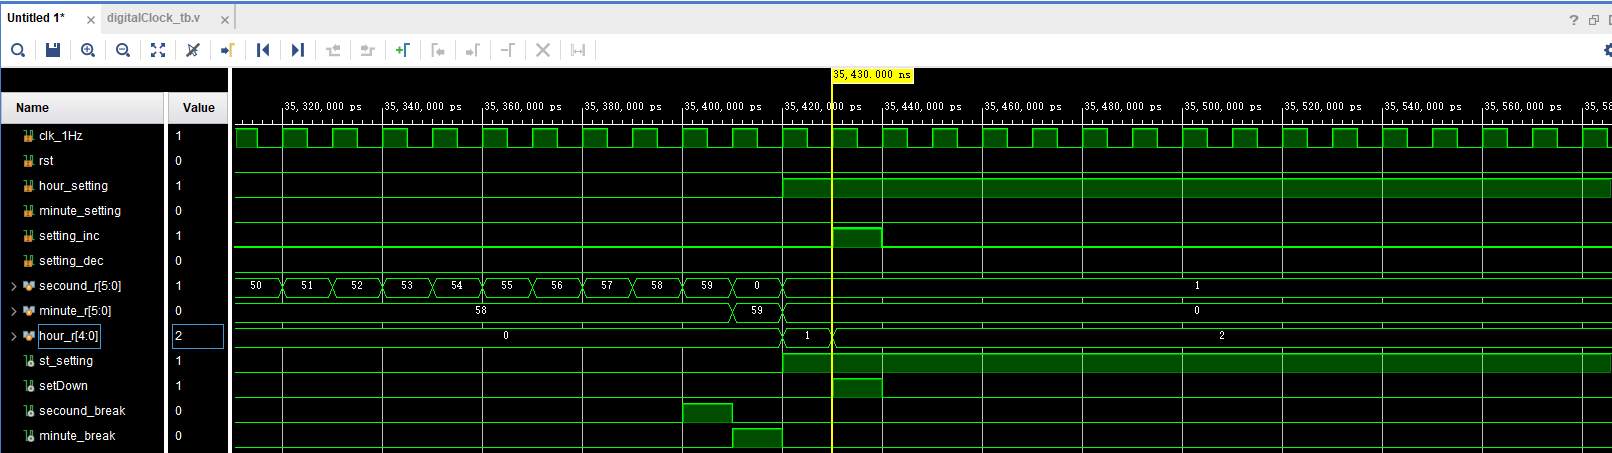
\includegraphics[width=0.7\textwidth]{image/2024-06-24-16-50-03.png}
    \caption{校准仿真}
    \label{image_base_sim_1}
\end{figure}
基础任务的计数功能工作正确, 复位按键可以实现秒计数的复位, 仿真图\ref{image_base_sim_1}中主要展示了通过按键
的形式完成分和时的校准, 可以看到在进入时校准的状态下, 一个inc的上升沿信号可以使得时计数器增加。\\
\newpage
\begin{figure}[htbp]
    \centering
    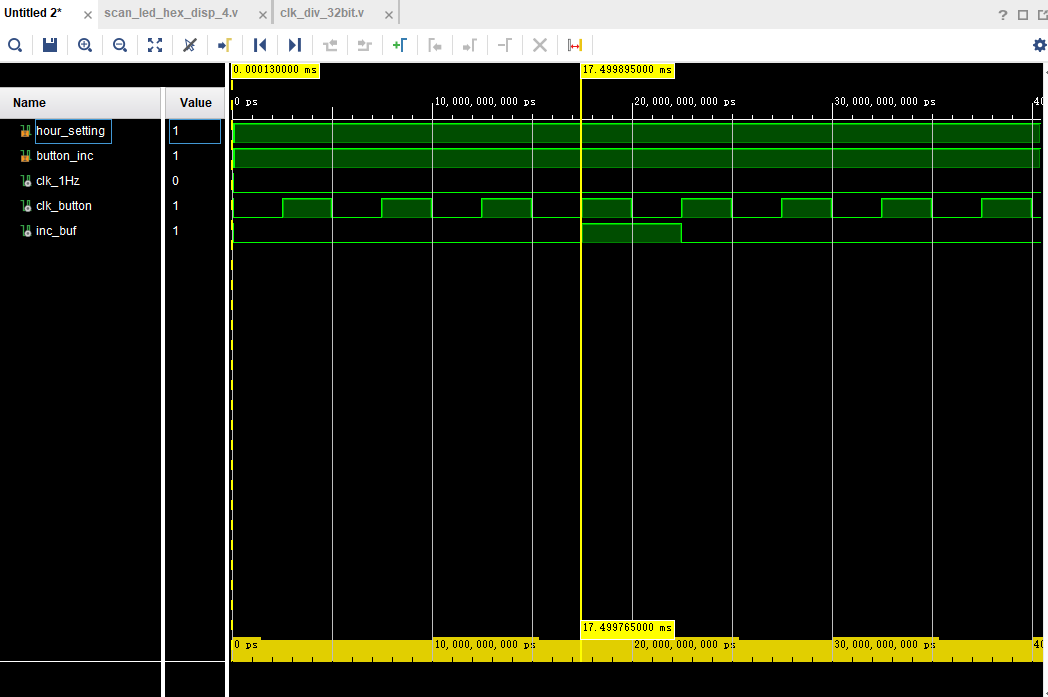
\includegraphics[width=0.5\textwidth]{image/2024-06-24-21-06-19.png}
    \caption{按键消抖仿真}
    \label{image_base_sim_2}
\end{figure}
按键消抖模块工作正常, 仿真图\ref{image_base_sim_2}可以看到按键消抖正常工作, 同时利用按键时钟
将异步的信号转化为同步信号进行模块间传输。\\

\begin{figure}[htbp]
    \centering
    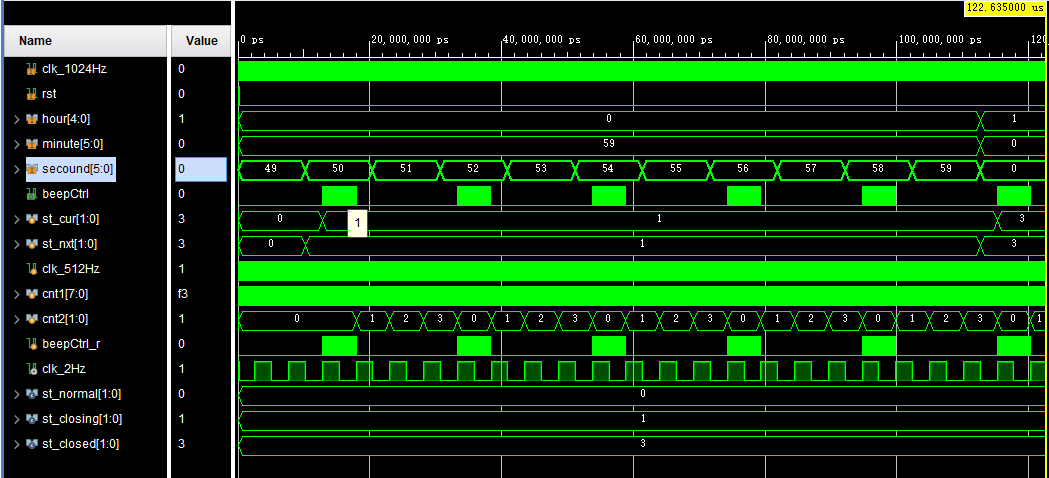
\includegraphics[width=0.7\textwidth]{image/2024-06-25-22-48-35.png}
    \caption{报时模块仿真}
    \label{image_tellTime_sim_1}
\end{figure}
报时模块的仿真结果如图\ref{image_tellTime_sim_1}所示, 当进入整点前的十秒钟时, 系统每两秒输出512Hz信号半秒
, 用于控制蜂鸣器输出报时信号, 最后进入整点时同样输出半秒信号, 将输出切换至1024Hz。\\

\begin{figure}[htbp]
    \centering
    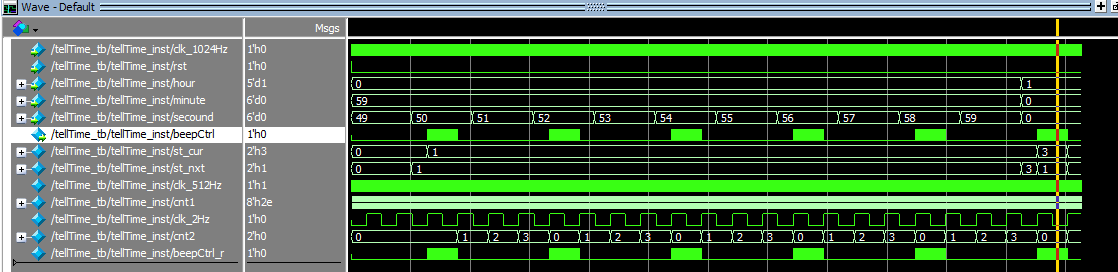
\includegraphics[width=0.7\textwidth]{image/2024-06-25-21-26-28.png}
    \caption{modelsim仿真结果}
    \label{image_tellTime_sim_2}
\end{figure}
通过modesim仿真结果如图\ref{image_tellTime_sim_2}, 可以更加清晰地看到不同的数据的详细信息。\\
\subsection*{拓展任务}
\begin{figure}[H]
    \centering
    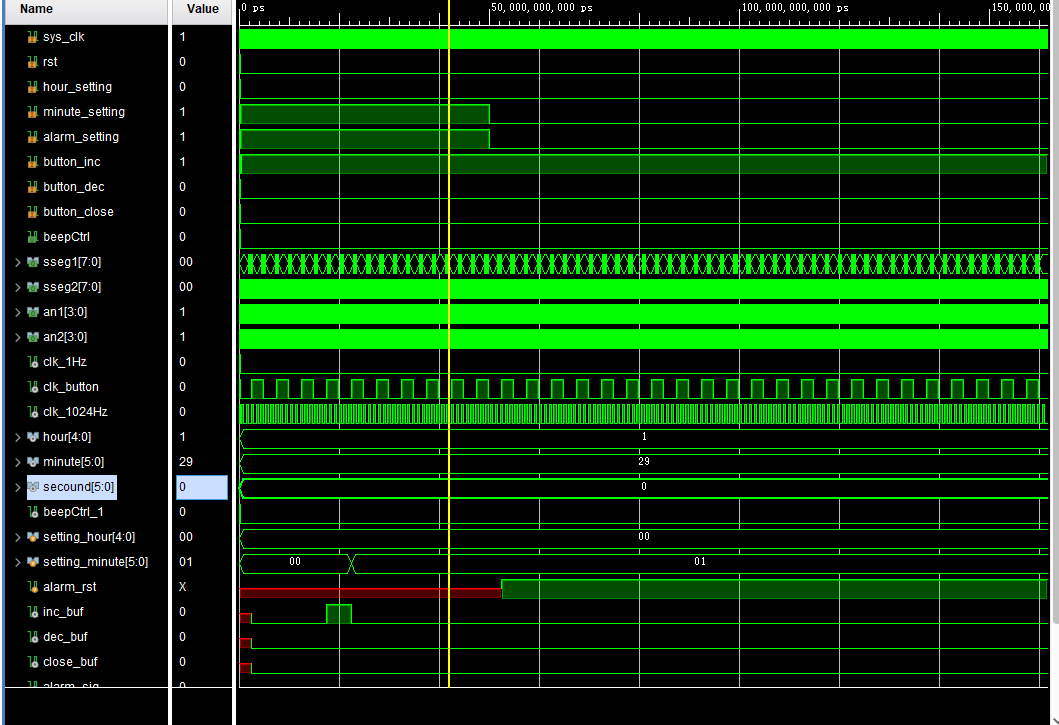
\includegraphics[width=0.6\textwidth]{image/2024-06-25-21-56-47.png}
    \caption{设置闹钟仿真}
    \label{image_alarm_sim_1}
\end{figure}
设置闹钟功能的仿真如图\ref{image_alarm_sim_1}所示, 通过增加按键, 成功使得预置计数器增加一;\\

\begin{figure}[htbp]
    \centering
    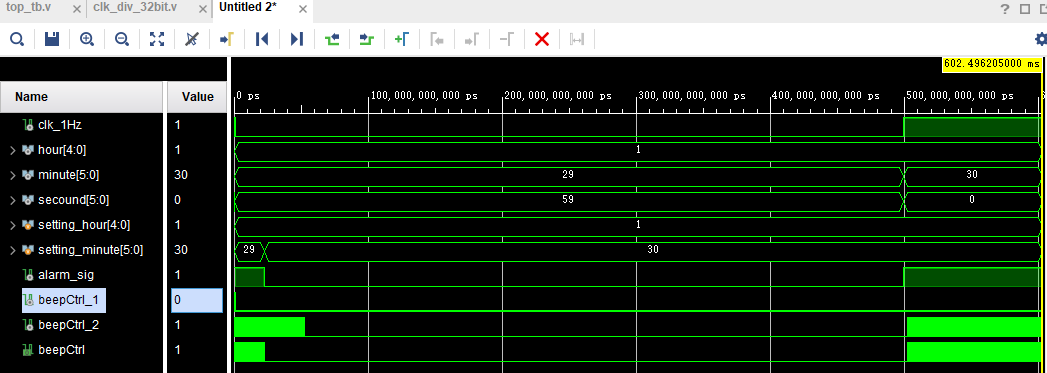
\includegraphics[width=0.7\textwidth]{image/2024-06-25-22-07-02.png}
    \caption{闹钟生效仿真}
    \label{image_alarm_sim_2}
\end{figure}
闹钟生效时的仿真结果如图\ref{image_alarm_sim_2}所示, 当设置结果同当前时间一致时蜂鸣器发声。\\

\begin{figure}[htbp]
    \centering
    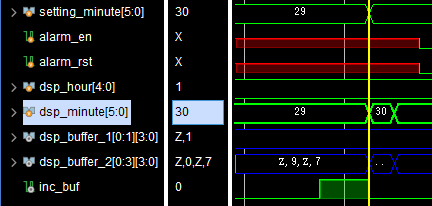
\includegraphics[width=0.7\textwidth]{image/2024-06-25-22-13-26.png}
    \caption{闹钟设置期间的显示仿真}
    \label{image_alarm_sim_3}
\end{figure}
闹钟设置期间的显示仿真如图\ref{image_alarm_sim_3}所示, 当进入闹钟设置模式时, 显示结果为预置计数器。\\
\begin{figure}[H]
    \centering
    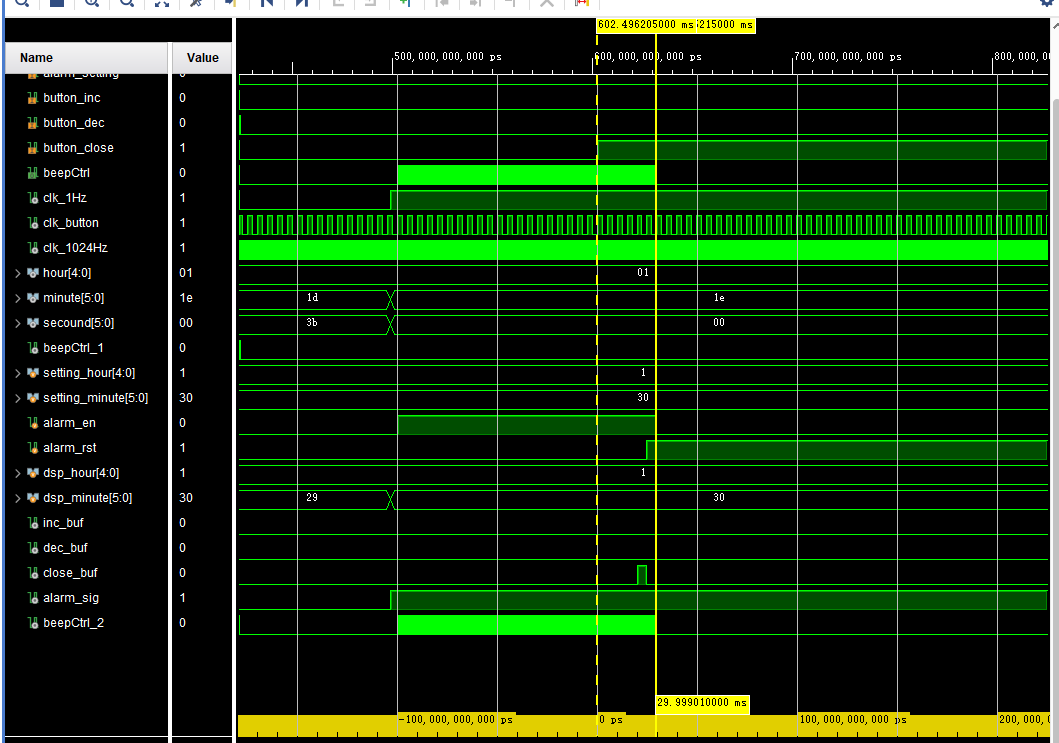
\includegraphics[width=0.7\textwidth]{image/2024-06-25-22-16-52.png}
    \caption{闹钟停止按键的仿真}
    \label{image_alarm_sim_4}
\end{figure}
闹钟停止按键的仿真结果如图\ref{image_alarm_sim_4}所示, 当按下停止闹钟按键后, 大概有30ms左右的延迟完
成闹钟关闭, 否则该闹钟会持续一分钟。\\
% 第四部分
\section*{\fourhao 四、硬件验证结果}
\xiaosihao
\setstretch{1.5}
% 记录加编程器与拨码开关和发光二极管、数码管等的连接情况。记录开发板硬件验证结果,并分析其结果的正确性。
% 按照基础任务、提高任务和拓展任务分别分析
\subsection*{基础任务}
\begin{figure}[H]
    \centering
    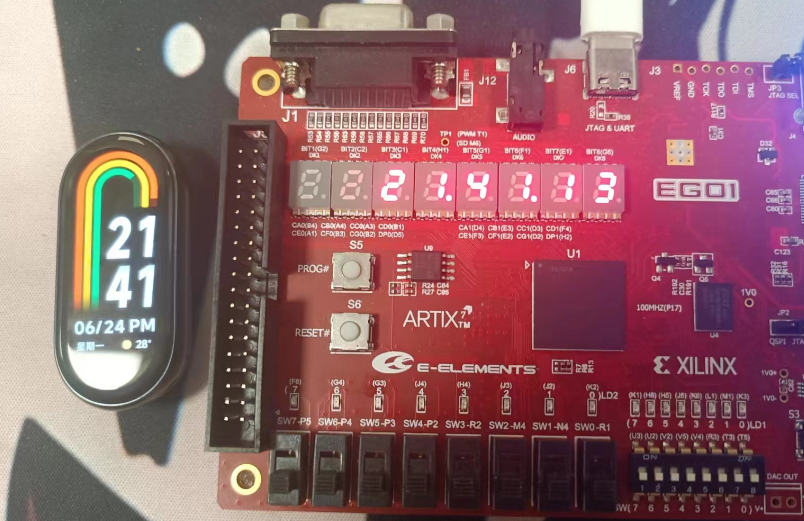
\includegraphics[width=0.5\textwidth]{image/2024-06-24-21-42-35.png}
    \caption{基础任务硬件验证结果}
    \label{image_verify_1}
\end{figure}
基础部分的三个功能验证结果如图\ref{image_verify_1}所示, 通过校时模式, 完成了分和时的校准并与现有手表进行对比, 
保证时间精确性, 通过复位按键复位秒计时器, 实现时间校准, 完成基础任务要求。\\
\subsection*{提高任务}
\begin{figure}[H]
    \begin{minipage}[t]{0.45\linewidth}
        \centering
        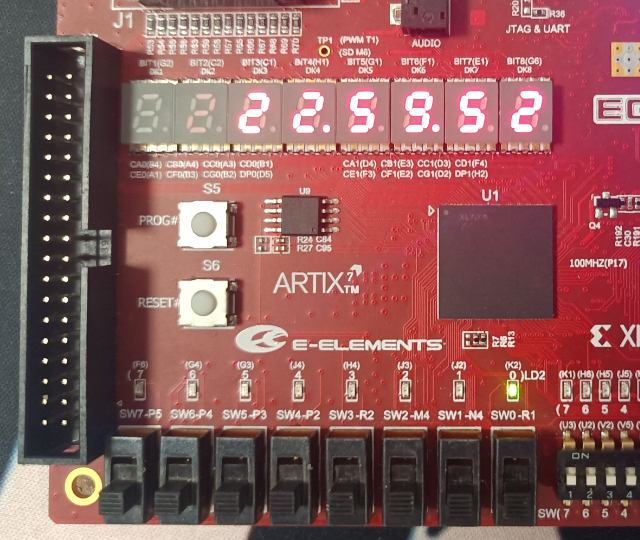
\includegraphics[width=0.7\textwidth]{image/2024-06-26-08-54-42.png}
        \caption{接近整点报时}
        \label{image_verify_2}
    \end{minipage}
    \begin{minipage}[t]{0.45\linewidth}
        \centering
        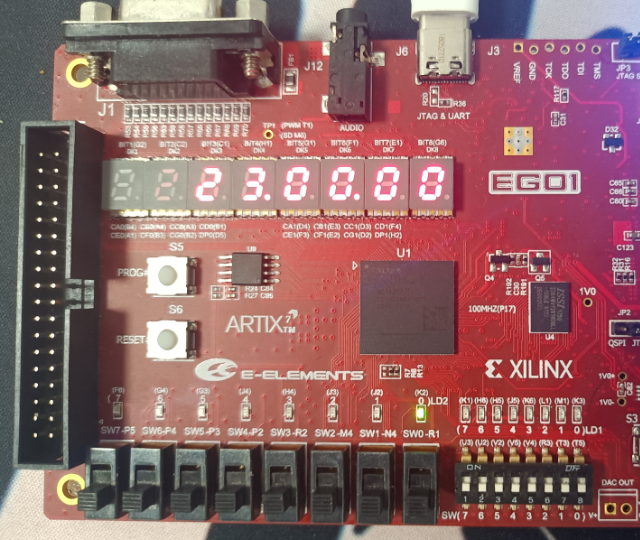
\includegraphics[width=0.7\textwidth]{image/2024-06-26-08-54-17.png}
        \caption{整点报时}
        \label{image_verify_3}
    \end{minipage}
\end{figure}
整点报时功能如图\ref{image_verify_2}和图\ref{image_verify_3}所示, 模块设计时输出信
号为512Hz或者1024Hz的方波用于驱动无源蜂鸣器, 但为了静态观察实验现象, 将输出结果约束至
LED灯LD2\_0上, 图\ref{image_verify_2}展示的是从22:59:50开始, 每隔两秒, led灯点亮0.5s,
但由于其频率为512Hz, 肉眼无法观察, 只能观察到灯被点亮。 图\ref{image_verify_3}展示的
到达整点报时, 此时led灯点亮0.5s, 输出1024Hz, 同样肉眼无法观察, 可以看到led灯点亮0.5s。
\subsection*{拓展任务}
\begin{figure}[H]
    \begin{minipage}[t]{0.3\linewidth}
        \centering
        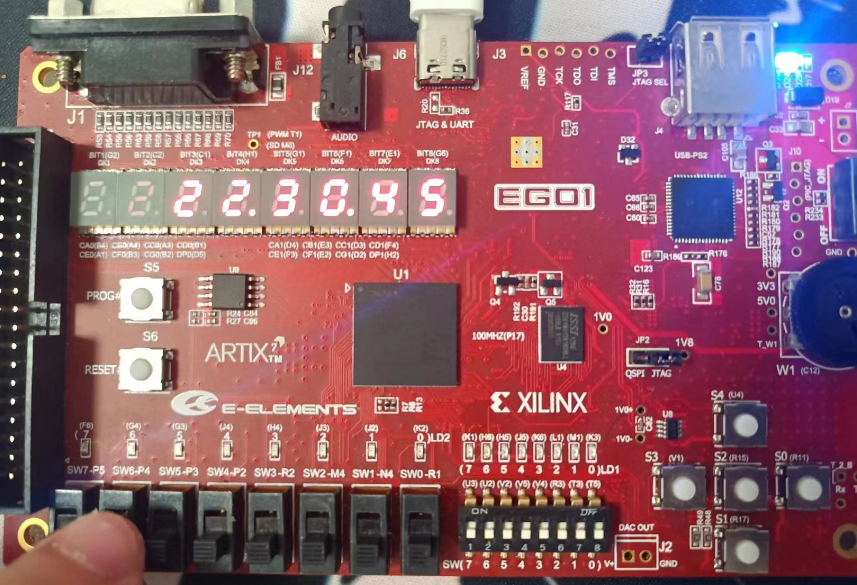
\includegraphics[width=0.7\textwidth]{image/2024-06-26-09-04-34.png}
        \caption{正常状态}
        \label{image_alarm_verify_1_1}
    \end{minipage}
    \begin{minipage}[t]{0.3\linewidth}
        \centering
        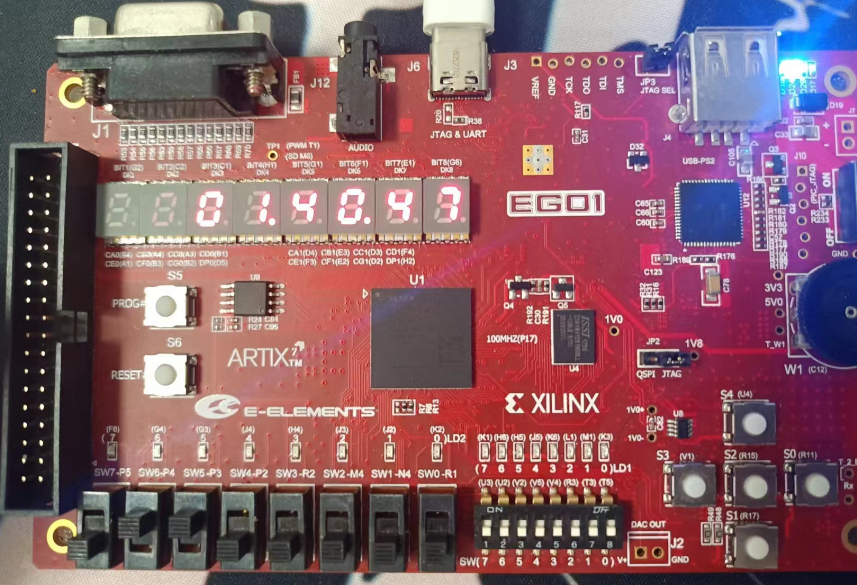
\includegraphics[width=0.7\textwidth]{image/2024-06-26-09-05-12.png}
        \caption{预置计数器}
        \label{image_alarm_verify_1_2}
    \end{minipage}
    \begin{minipage}[t]{0.3\linewidth}
        \centering
        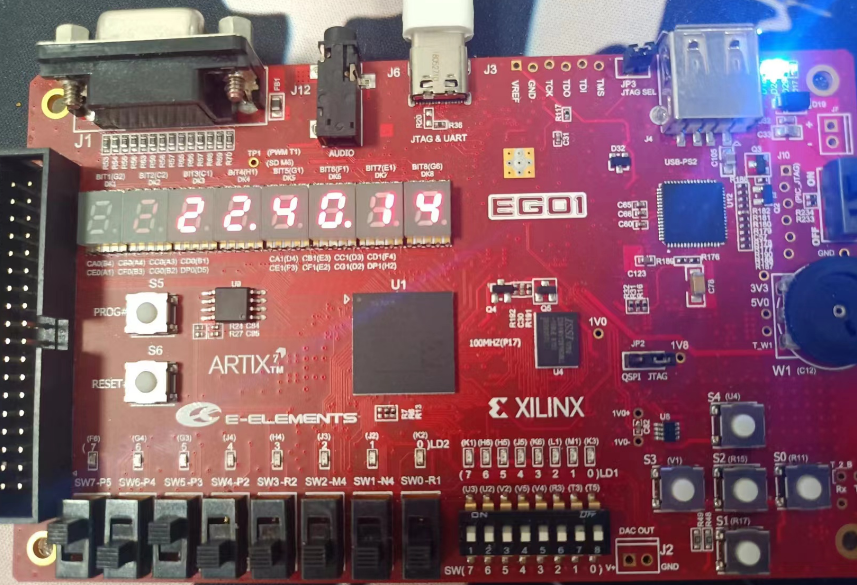
\includegraphics[width=0.7\textwidth]{image/2024-06-26-09-05-49.png}
        \caption{设置闹钟结果}
        \label{image_alarm_verify_1_3}
    \end{minipage}
\end{figure}
设置闹钟的过程如图\ref{image_alarm_verify_1_1}、图\ref{image_alarm_verify_1_2}和图\ref{image_alarm_verify_1_3}所示, 
其中图\ref{image_alarm_verify_1_1}展示了默认状态下的时钟情况,\ref{image_alarm_verify_1_2}是进入了闹钟设置状态, 可见其
预置计数器内容与时钟不一致, 通过设置改变预置计数器内容, 设置闹钟结果如图\ref{image_alarm_verify_1_3}所示。\\
\begin{figure}[H]
    \begin{minipage}[t]{0.45\linewidth}
        \centering
        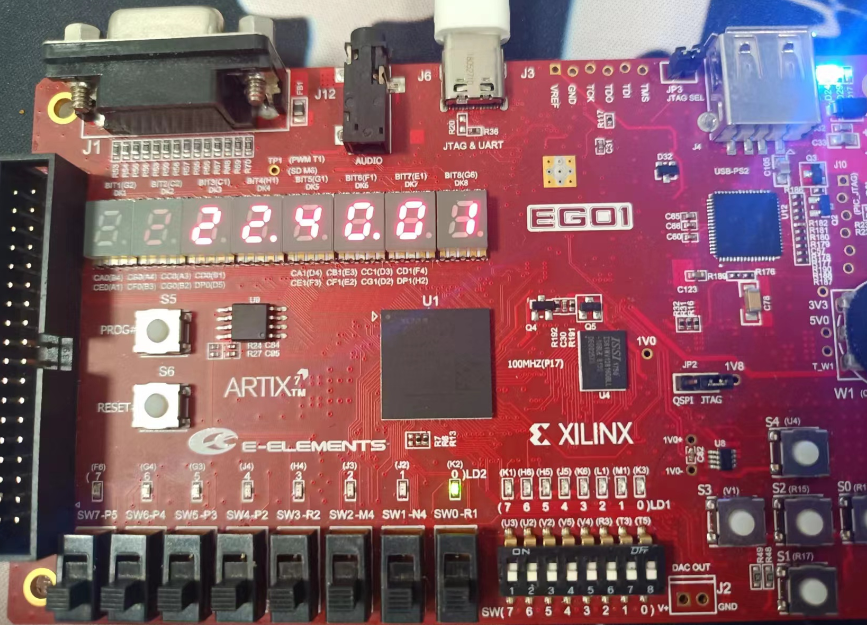
\includegraphics[width=0.7\textwidth]{image/2024-06-26-09-09-13.png}
        \caption{闹钟触发}
        \label{image_alarm_verify_2_1}
    \end{minipage}
    \begin{minipage}[t]{0.45\linewidth}
        \centering
        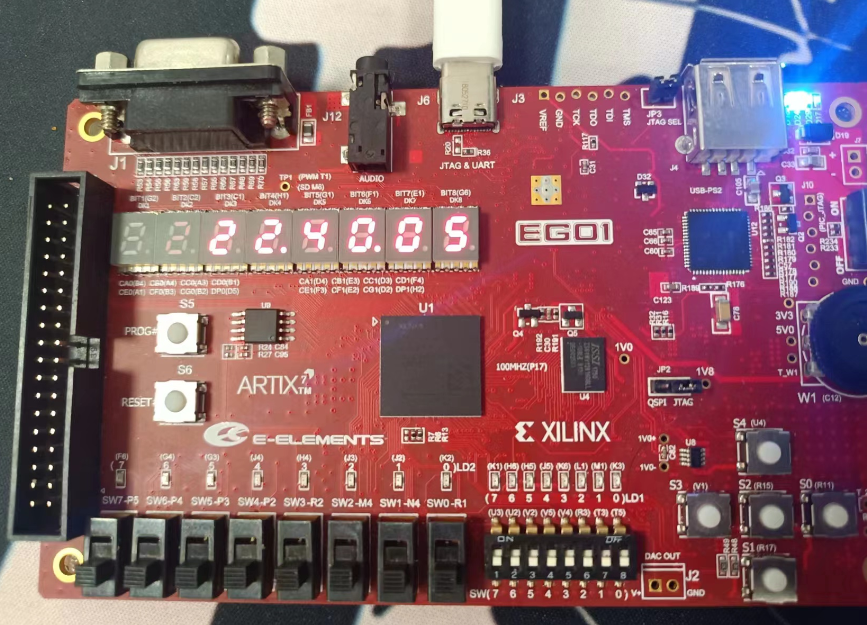
\includegraphics[width=0.7\textwidth]{image/2024-06-26-09-09-39.png}
        \caption{通过按键关闭闹钟}
        \label{image_alarm_verify_2_2}
    \end{minipage}
\end{figure}
闹钟触发的过程如图\ref{image_alarm_verify_2_1}和图\ref{image_alarm_verify_2_2}所示, 当时间到达如图\ref{image_alarm_verify_1_3}所示设置的22:40分闹钟时,
led灯被点亮, 输出1024Hz的信号驱动蜂鸣器, 如果不按下关闭闹钟按键的话, 该闹钟将持续1分钟, 如图\ref{image_alarm_verify_2_2}
所示为提前按下关闭按键, 闹钟被关闭, LED灯熄灭。 
% 第五部分
\section*{\fourhao 五、问题解决}
\xiaosihao
\setstretch{1.5}
% 设计过程中遇到的问题及解决的方法。
\subsection*{无法实现always语句块的异步赋值}
解决: 在使用计数器完成校时功能时, 虽然仿真和代码无误, 但硬件验证结果并不理想, 按键无效。\\
\begin{figure}[H]
    \centering
    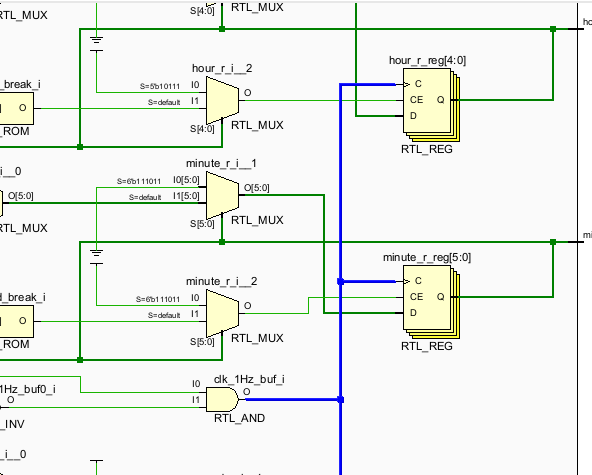
\includegraphics[width=0.5\textwidth]{image/2024-06-24-19-51-58.png}
    \caption{发现问题的原理图}
    \label{image_QA_1}
\end{figure}
综合结果如图\ref{image_QA_1}所示, 对触发器进行赋值时, 虽然敏感列表写了inc和dec信号, 但其并未被综合到触发器的触发端, 
但其相应的组合逻辑功能有被正确的综合, 在进行仿真的过程中, 并不会进行任何优化, 所以不会发生错误。\\

问题出在如何让定时器能够有效的接收异步的按键信号, 并进行加或者减法, 因此, 通过引入按键的消抖状态机解决问题, 
同时为按键信号引入伴随时钟, 实现按键信号和计数器模块间的同步传输。
\subsection*{已添加消抖模块, 但设计得到的数字钟按键会突然使数据增加数次}
\begin{figure}[htbp]
    \centering
    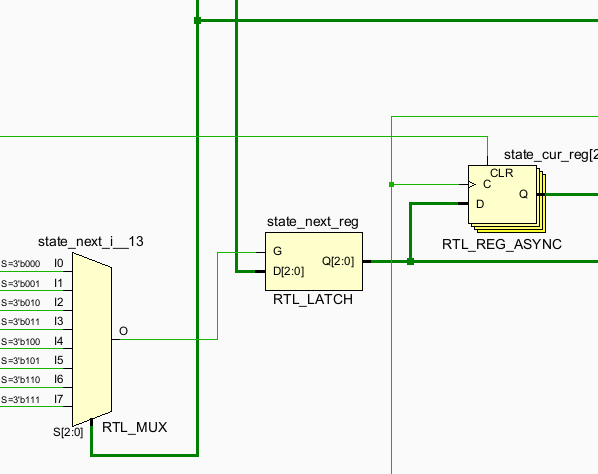
\includegraphics[width=0.5\textwidth]{image/2024-06-24-22-21-16.png}
    \caption{错误综合结果}
    \label{image_QA_2}
\end{figure}
消抖模块经过验证无误, 认为问题并不出在消抖上, 检查综合结果发现问题, 见图\ref{image_QA_2}, 本来应
该是组合逻辑的状态转移求解次态的电路中综合出了latch, 导致消抖模块的状态混乱, 频繁输出按键有效信号, 
导致了按键抖动现象。\\

直接通过右键latch, 可以直接查看对应的综合代码, 发现是求解次态电路中
误删了次态默认等于当前状态, 导致if-else语句结构不完整, 综合产生LATCH, 修改后解决问题。
\subsection*{时钟寄存器无复位要求难以仿真}
由于时钟寄存器要求无复位, 其初值无法指定, 就算可以复位, 也无法很方便的设定任意初值用于仿真, 通过查阅资料得知, 可以在模块内通过写无法综合的语句辅助进行仿真, 如initial语句块等, 在进行仿真时可以有效的方便仿真。
% 第六部分
\section*{\fourhao 六、心得体会}
\xiaosihao
首次独立完成较为复杂的项目, 花费众多时间进行设计和仿真, 尤其是仿真阶段耗费大量时间来使得设计结果科学合理, 
能够证明设计无误, 期间为了能够尽快完成秒级的仿真初步接触了modelsim仿真工具, 在本次实验中进一步提高了对仿真工具的运用能力。\\

第一次在一个设计中使用如此多的时钟, 体会到复杂系统, 如arm内核的MCU中时钟树设计的意义, 能够在最大程度上提高
时钟资源的利用率的同时, 还能保证不同模块间的同步运行, 在日后再次进行复杂设计时可以借鉴此思路, 在设计前首先构建模块框图, 
使尽量多的模块能够同步工作, 减小异步模块间的联系, 简化系统。\\

通过6次实验设计的锻炼, 逐渐熟练对综合工具的应用, 出现问题后可以迅速定位, 并进一步的在设计时避免综合工具的问题, 本次
实验中在基础部分还会花一定的时间用在解决综合工具问题上, 但是在提高和拓展部分在设计时有意识地避免综合问题, 将大部分时间花在仿真上, 
仿真无误后进行烧录一次成功。\\
\end{document}
